\chapter{Galaxy selection using the thermal Sunyaev-Zeldovich effect (a way beyond 2-point)\texorpdfstring{\footnote{This chapter is work in progress, to be published as \cite{tSZ-selection-DESI-LRGs}}}{}}
\label{ch:tSZ-selection-LRG}
\graphicspath{{tSZ-selection-LRG/}}

\section{Introduction}

Modern cosmology is a high-precision science thanks to a rich variety of data collected.
The large-scale structure of the Universe contributes a major portion of this data.
Most important techniques include baryon acoustic oscillations distance measurements \citep[e.g.,][]{DESI.DR2.BAO.lya,DESI.DR2.BAO.cosmo} and full-shape clustering analyses \citep{DESI2024.V.KP5,DESI2024.VII.KP7B}, both based on galaxy redshift surveys.

Looking into the future, it is important to determine priorities for the next spectroscopic surveys.
The expansion towards higher redshifts is well motivated by the primordial Universe studies.
However, observations pose new challenges as spectral features of galaxies redshift out of the near-visible range accessible to ground-based telescopes \citep{snowmass2021-high-z-LSS}.

In contrast, measuring more galaxy spectra at lower redshifts is easier technically.
We already have a dense sample in the DESI Bright Galaxy Survey (\cite{BGS.TS.Hahn.2023}).
Only a small portion of it is used for the BAO and full-shape analyses \citep{DESI2024.III.KP4,DESI2024.V.KP5,DESI.DR2.BAO.cosmo}.
In the future DESI upgrade, DESI-II, the density of the luminous red galaxy (LRG) sample will also increase greatly \citep{spectroscopic-roadmap-cosmic-frontier}.
However, the scientific case for such higher-density samples is not so clear and specific.

There are promising ideas for leveraging information from different galaxy environments that can benefit from dense samples.
One is density-marked clustering, which assigns additional weight to galaxies based on a local density estimate at their location.
It was originally introduced in \cite{density-marked-CF-MG} to enhance modified gravity tests,
and was later tuned to give tighter constraints on neutrino mass \citep{density-marked-PS-neutrinos} and other cosmological parameters \citep{density-marked-PS-cosmoinfo,density-marked-PS-SBI}.
Another is density-split clustering, which splits galaxies into subsamples based on the local density estimate.
It was introduced for better modeling of redshift-space distortions in \cite{density-split-clustering-RSD}.
Later works predict tighter constraints on standard cosmological parameters and neutrino masses \citep{density-split-clustering-constrain-nuLCDM}, or primordial non-Gaussianity \citep{density-split-clustering-PNG}.
A simulation-based model of density-split clustering was built \citep{density-split-clustering-sim-based-model} and applied to BOSS CMASS data \citep{density-split-clustering-BOSS-CMASS}, surpassing the standard analysis.

A number of works demonstrated the benefit of combining galaxy redshift surveys with data on secondary cosmic microwave background (CMB) anisotropies, particularly lensing.
For example, \cite{ACT-lensingxDESI-LRG-structure-formation-Kim,ACT-lensingxDESI-LRG-structure-formation-Sailer} cross-correlate lensing with spectroscopic galaxies to better constrain the growth of cosmic structure, and \cite{DESI-QSOxPlanck-lensing-PNG,DESI-LRGxPlanck-lensing-PNG} improve measurements of primordial non-Gaussianity.
This combination of probes is very promising, because DESI is taking galaxy spectra at an unprecedented rate, and the next CMB experiments like Simons Observatory \citep{SO} and CMB-S4 \citep{CMBS4,CMBS4white} have great prospects for secondary CMB anisotropies, including lensing and Sunyaev-Zeldovich effects.

We decided to use the thermal Sunyaev-Zeldovich (tSZ) effect.
It is inverse Compton scattering of cosmic microwave background (CMB) photons on free thermal electrons moving randomly (whereas bulk motions give rise to the kinetic or kinematic Sunyaev-Zeldovich effect).
This process results in a net increase in energy of scattered photons and creates a distinct frequency-dependent distortion in the CMB spectrum.
The relative change in photon energy is approximately equal to the Compton $y$ parameter, which is proportional to the integral of free electron density $n_e$ and temperature $T_e$ along the path \citep[with length element $dr$;][]{Planck-SZ-map,Sunyaev-Zeldovich-1972}:
\begin{equation} \label{eq:y-parameter-0}
    y = \int \frac{k_B T_e}{m_e c^2} n_e \sigma_T dr,
\end{equation}
other quantities are constants: electron rest mass energy $m_e c^2$, Boltzmann's constant $T_e$ and Thomson scattering cross-section $\sigma_T$.
Accordingly, the effect is strongest in ionized, hot and dense gas in or around galaxy clusters \citep[as suggested by][]{Sunyaev-Zeldovich-1970,Sunyaev-Zeldovich-1980-review}.
The clusters represent a distinct environment.

The tSZ data comes from CMB telescopes independent of DESI, whereas density estimates depend on the galaxy observation strategies.
Using different datasets would allow us to check their consistency, check for systematics and potentially discover new fundamental tensions.
Specific improvements could include
testing the conformity of different galaxy sub-types \citep[e.g.,][]{LSS-color-dependent-stochasticity},
improving the redshift-space distortion modeling for full-shape clustering analyses by removing a small fraction of the strongest Fingers of God \citep{removing-FoG},
obtaining multiple tracers with better-constrained biases for the primordial non-Gaussianity measurements \citep[similarly to][]{multi-tracer-PNG-forecasts}
or constraining environmental effects on galaxy formation or galaxy-halo connection \citep[e.g.,][]{EDR_HOD_LRGQSO2023}.

We need to remark that Sunyaev-Zeldovich maps have been used for cluster studies: their detection, mass determination, and more \citep{Planck-SZ-clusters,ACT-SZ-clusters-DR5,ACT-SZ-clusters-mass-calibration-DR5,SPT-clusters-w-DES+HST-WL,SPT-SZ-clusters-2025}.
But rigorously detected and confirmed cluster candidates are rare.
We aim to extract more information from the lower signal-to-noise parts, which comprise a much bigger fraction of the map.

This work is not going to provide the final answers and methodology, but rather motivate further developments.
It is structured as follows:
\cref{sec:DESI-tSZ:data} introduces the data and simulations we use,
\cref{sec:DESI-tSZ:measurements} details our processing of real data and provides its results,
\cref{sec:DESI-tSZ:mock} describes our simulation-based toy model, compares it with data and shows new insights,
\cref{sec:DESI-tSZ:conclusions} concludes with a summary and a future outlook.

\section{Data}
\label{sec:DESI-tSZ:data}

\subsection{Galaxy catalog: DESI DR1 LRG}

The Dark Energy Spectroscopic Instrument (DESI) \citep{DESI2016a.Science,DESI2022.KP1.Instr} conducts a 5-year galaxy redshift survey.
Its scientific program has been successfully validated \citep{DESI2023a.KP1.SV} alongside the Early Data Release \citep{DESI2023b.KP1.EDR}.
The key results based on Data Release 1 \citep[recently made public]{DESI2024.I.DR1} include clustering catalogs and two-point statistics measurements \citep{DESI2024.II.KP3}, baryon acoustic oscillation (BAO) distance measurements from galaxies, quasars \citep{DESI2024.III.KP4} and Lyman-$\alpha$ forest \citep{DESI2024.IV.KP6} along with their detailed implications for cosmological models \citep{DESI2024.VI.KP7A}; and full-shape clustering of galaxies and quasars \citep{DESI2024.V.KP5} with their cosmological analysis \citep{DESI2024.VII.KP7B}.
Furthermore, updated BAO measurements from Lyman-$\alpha$ \citep{DESI.DR2.BAO.lya}, galaxies and quasars with accompanying cosmological interpretations \citep{DESI.DR2.BAO.cosmo} are also available, based on Data Release 2 \citep{DESI.DR2.DR2}.

We use Luminous Red Galaxies \citep[LRG;][]{LRG.TS.Zhou.2023} from the DESI DR1 clustering catalog \citep{DESI2024.II.KP3,DESI2024.I.DR1}.
We chose LRG because their redshift range ($0.4<z<1.1$) covers the peak in redshift distribution of Sunyaev-Zeldovich clusters \citep{ACT-SZ-clusters-DR5}.
We discard galaxies at $z>0.85$ because then both the LRG density \citep{DESI2024.II.KP3} and the SZ cluster abundance \citep{ACT-SZ-clusters-DR5} drop.

\subsection{Sunyaev-Zeldovich map: ACT DR6}

The Atacama Cosmology Telescope \citep[ACT;][]{ACT-design,ACT} was a ground-based cosmic microwave background (CMB) experiment.
Compared to the space-based {\it Planck} mission \citep{planck_overview}, it has a smaller sky fraction, but reaches small angular scales thanks to higher resolution, and measures the CMB polarization with higher precision due to lower instrumental noise.
Both of these are very important for Sunyaev-Zeldovich analyses.

We use the thermal Sunyaev-Zeldovich Compton $y$ parameter map from ACT DR6 \citep{ACT-maps-DR6}.
We rely on the accompanying noise simulations \citep{ACT-noise-simulations-DR6} to estimate the signal-to-noise ratio in our analysis.

\subsection{Simulations: \abacussummit{} halo catalogs}

We also use a $z=0.8$ snapshot of a $\qty(2\ihGpc)^3$ cubic box (for the fiducial cosmology) from the \abacussummit{} suite of $N$-body simulations \citep{AbacusSummit} produced with \abacus{} code \citep{Abacus-code}.
The halos have been identified with the \compaso{} halo finder \citep{CompaSO-halo-finder}.
We use a galaxy catalog produced within the halo occupation distribution (HOD) galaxy-halo connection framework, efficiently implemented in \abacushod{} \citep{AbacusHOD} with parameters based on \cite{EDR_HOD_LRGQSO2023}.
This galaxy catalog was one of the base cubic boxes for {\tt Abacus-2} cut-sky mocks described in \cite{DESI2024.III.KP4}.

\section{Measurements}
\label{sec:DESI-tSZ:measurements}

\subsection{Methodology and challenges}
\label{sec:DESI-tSZ:measurements:methodology}

We divide the LRGs into subsamples (``SNR bins'') according to the signal-to-noise ratio at their location in the ACT DR6 + {\it Planck} $y$ map \citep{ACT-maps-DR6}.
First, we match the positions of the LRGs from the DESI clustering catalog to the pixels in the map.
Second, we compute the pixel-level standard deviations in $y$ using the corresponding 304 Gaussian noise simulation \citep{ACT-noise-simulations-DR6}.
Finally, we compute the signal-to-noise ratio in each pixel by dividing the $y$ value by its standard deviation.

Such external selection of galaxies imposes complex geometry changes that affect the estimation of the clustering statistics.
E.g., the Landy-Szalay estimator \citep{Landy-Szalay} for the correlation function between samples 1 and 2 (which may be identical or different):
\begin{equation} \label{eq:2PCF-Landy-Szalay}
    \hat \xi^{\rm LS}_{12} = \frac{D_1 D_2 - D_1 R_2 - R_1 D_2}{R_1 R_2} + 1,
\end{equation}
where $D_1 D_2$ are the (binned) pair counts between data (galaxies) from sample 1 and data 2, $D_1 R_2$ are the pair counts between data 1 and random points (reflecting the survey geometry and selection etc) for sample 2, $R_1 D_2$ are between random points 1 and data 2, and $R_1 R_2$ are between random points 1 and 2.

The key to the problem is that the full-survey random catalogs are not representative of our subsamples.
One might think that imposing the same on-sky position filter on random points would be a solution, however, it is not perfect.
The resulting randoms would be (narrow) columns extended along the line of sight, whereas a significant portion of selected galaxies would be truly clumped around the cluster position in 3 dimensions.

It is possible to leave the unusually-looking clustering measurement and model it consistently.
But we have decided to keep the correlation functions more intuitive.
To achieve this, we avoid the issue with the subsample geometry by employing an asymmetric Davis-Peebles estimator \citep{Davis-Peebles} for the correlation function:
\begin{equation} \label{eq:2PCF-Davis-Peebles}
    \hat \xi^{\rm DP}_{12} = \frac{D_1 D_2}{D_1 R_2} - 1.
\end{equation}
The $D_1 D_2$ and $D_1 R_2$ are the same pair counts as in the Landy-Szalay estimator (\cref{eq:2PCF-Landy-Szalay}).
However, we note that the randoms representing sample 1 are not required: neither $R_1 D_2$ nor $R_1 R_2$ are involved.
The randoms are only necessary for sample 2.
Therefore, with this estimator, we can compute the correlation function between the tSZ subsample (as 1) and the full LRG sample (as 2).

We also apply filters to the $y$ map for two reasons.
First, a filter matched to a cluster SZ profile would optimally detect them and recover their positions \citep{matched-filters-intro}.
Second, the environmental influence of a cluster is likely to extend further than its Compton parameter profile.
Our fiducial filter is not thoroughly matched, but has a Gaussian shape with a 2.4 arcmin full width at the half-maximum for simplicity.
The single filter in the ACT DR5 catalog paper has the same scale \citep{ACT-SZ-clusters-DR5}.
We apply the same filter to all the noise simulations to obtain the corresponding pixel-wise standard deviation map.

\subsection{Larger-scale clustering and galaxy bias}
\label{sec:DESI-tSZ:measurements:large}

First, we compute the larger-scale cross-correlation functions between the different SNR bins and the full LRG sample.
We use the radial ($s$) and angular ($\mu$) binning.
We disregard the pairs located too closely on the sky\footnote{This is technically known as the theta ($\theta$) cut.} for two reasons.
The first is to avoid using pairs of galaxies belonging to the same SZ pixel, or associated with the same line of sight smeared by the beam and the filter.
The second is to mitigate the DESI fiber assignment incompleteness effects \citep{KP3s5-Pinon}.
We only count pairs with the angular separation above 0.1 degrees (6 arcmin)\footnote{This leaves $\mu\approx 1$ bins with no pair counts and undefined correlation functions. We discard these bins and average over the remaining bins to obtain the correlation function monopole.}.

We show the resulting isotropic cross-correlation functions in \cref{fig:clustering-SNR-bins} with covariances estimated using the jackknife technique.
We see a significant clustering enhancement in the monopole as the tSZ detection level increases, even though we stop at $4\sigma$, which was the threshold for cluster candidates in \cite{ACT-SZ-clusters-DR5}\footnote{However, bear in mind the simplicity of our filter, the matched filters of \cite{ACT-SZ-clusters-DR5} should be more optimal.}.
This almost certainly corresponds to an increase in galaxy bias.
0 to 1 $\sigma$ subsample appears very similar to the full LRG sample (as will continue to hold in many other respects).
For reference, \cref{tab:galaxy-numbers-SNR-bins} provides the number of galaxies in each SNR bin.

We should remark on the negative signal we obtain, contradicting the theoretical definition of the tSZ Compton $y$ parameter (\cref{eq:y-parameter-0}).
Instrumental (or atmospheric) noise plays a certain part.
Kinematic Sunyaev-Zeldovich effect, resulting from the bulk motions of free electrons, can have different signs and can become partially confused with ``negative'' thermal effect.
Other components, like the cosmic infrared background, may also leak into the thermal Sunyaev-Zeldovich reconstruction, potentially adding negative signal \citep{ACT-maps-DR6}.

\begin{figure}[htbp]
    \centering
    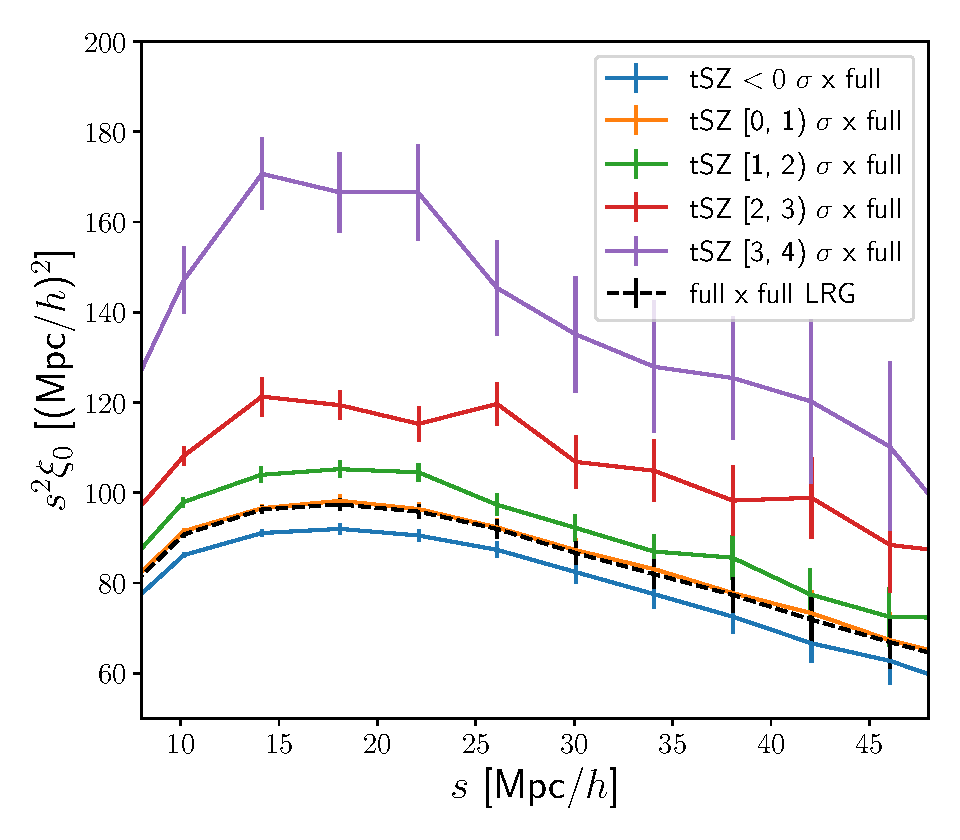
\includegraphics[width=\linewidth]{fig/LRG-z0.4-0.85-SZ-ACTPlanck-filtered2.4-monopole-jack-errorbars-clean.pdf}
    \caption[Large-scale cross-correlation functions of different tSZ SNR bins with the full LRG sample]{Large-scale isotropic (monopole) cross-correlation functions of different SNR bins with the full LRG sample.
    (Hereafter, we apply our fiducial Gaussian filter to the tSZ $y$ parameter map, and use the jackknife technique to estimate errorbars.)
    There is a significant clustering enhancement with increasing tSZ detection level even below the threshold for cluster candidates \citep[$4\sigma$ in][]{ACT-SZ-clusters-DR5}.}
    \label{fig:clustering-SNR-bins}
\end{figure}

\begin{table}[htbp]
    \centering
    \begin{tabular}{|r|r|}
        \hline
        SNR bin & $N_{\rm LRG}$ \\
        \hline
        $(-\infty, -2)$ $\sigma$ & 25101 \\
        $[-2, -1)$ $\sigma$ & 130331 \\
        $[-1, 0)$ $\sigma$ & 308498 \\
        $[0, 1)$ $\sigma$ & 305819 \\
        $[1, 2)$ $\sigma$ & 127875 \\
        $[2, 3)$ $\sigma$ & 25469 \\
        $[3, 4)$ $\sigma$ & 3577 \\
        $[4, 5)$ $\sigma$ & 981 \\
        $[5, 6)$ $\sigma$ & 484 \\
        $[6, \infty)$ $\sigma$ & 676 \\
        \hline
        Total & 928811 \\
        \hline
    \end{tabular}
    \caption[Number of galaxies in our tSZ SNR bins]{Number of DESI DR1 LRGs ($0.4<z<0.85$ and in the overlap with ACT footprint) in different tSZ SNR bins.}
    \label{tab:galaxy-numbers-SNR-bins}
\end{table}

For clarity, we seek to summarize each line in \cref{fig:clustering-SNR-bins} with a single number.
A simple way is to find the scaling for the full LRG correlation function to best match the cross-correlation function with any given signal-to-noise bin.
This multiplier should be similar to the ratio of the linear galaxy biases between the SNR subsample and the full LRG sample.
Accordingly, we also refer to this scaling as relative galaxy bias.

The jackknife covariance estimates for each correlation function allow us to estimate the precision of the scaling.
However, we have not estimated the covariances between different cross-correlation functions shown in \cref{fig:clustering-SNR-bins} consistently.
This makes our relative bias errorbar estimates imperfect and approximate.

We show the resulting galaxy biases of our subsamples (relative to the full LRG sample) in \cref{fig:relbias-SNR-bins}.
The picture is consistent with the conclusions we have drawn from \cref{fig:clustering-SNR-bins}: the increase of galaxy bias with the tSZ detection level, and the 0 to 1 $\sigma$ bin being close to average over all LRGs.
In addition, we can inspect more categories at negative signal-to-noise, different from the full LRG but not so significantly deviating from each other.

\begin{figure}[htbp]
    \centering
    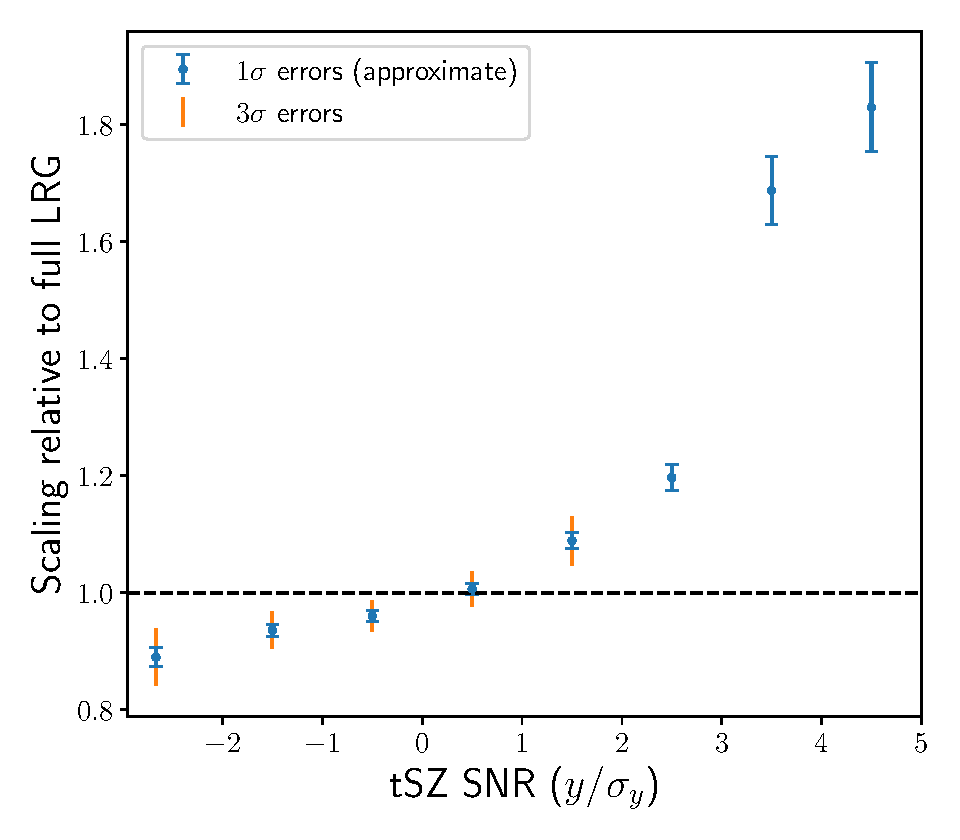
\includegraphics[width=\linewidth]{fig/LRG-z0.4-0.85-SZ-ACTPlanck-filtered2.4-monopole-jack-errorbars-relbias.pdf}
    \caption[Galaxy bias of different SNR bins relative to the full LRG sample]{Galaxy bias of different SNR bins relative to the full LRG sample.
    The bias increase (clustering enhancement) consistent with \cref{fig:clustering-SNR-bins} can be seen more concisely.}
    \label{fig:relbias-SNR-bins}
\end{figure}

\subsection{Small-scale line-of-sight clustering and velocity dispersions}
\label{sec:DESI-tSZ:measurements:small-LoS}

The cluster (supercluster) peculiar velocities are most apparent in configuration space at small scales near the line of sight.
Here we switch from $s$ and $\mu$ to the line-of-sight ($\pi$) and the perpendicular (on-sky, $r_p$) separations between the galaxy pair members.

Accordingly, we plot the line-of-sight small-scale correlation functions for our SNR bins in \cref{fig:LoS-clustering-SNR-bins}.
We notice an increase in correlation functions with the tSZ detection level in each bin, similar to the trends in larger-scale correlation functions (\cref{fig:clustering-SNR-bins}).
More interestingly, the slopes of the curves are also noticeably different, although it is hard to judge the significance of these differences visually.

\begin{figure}[hbtp]
    \centering
    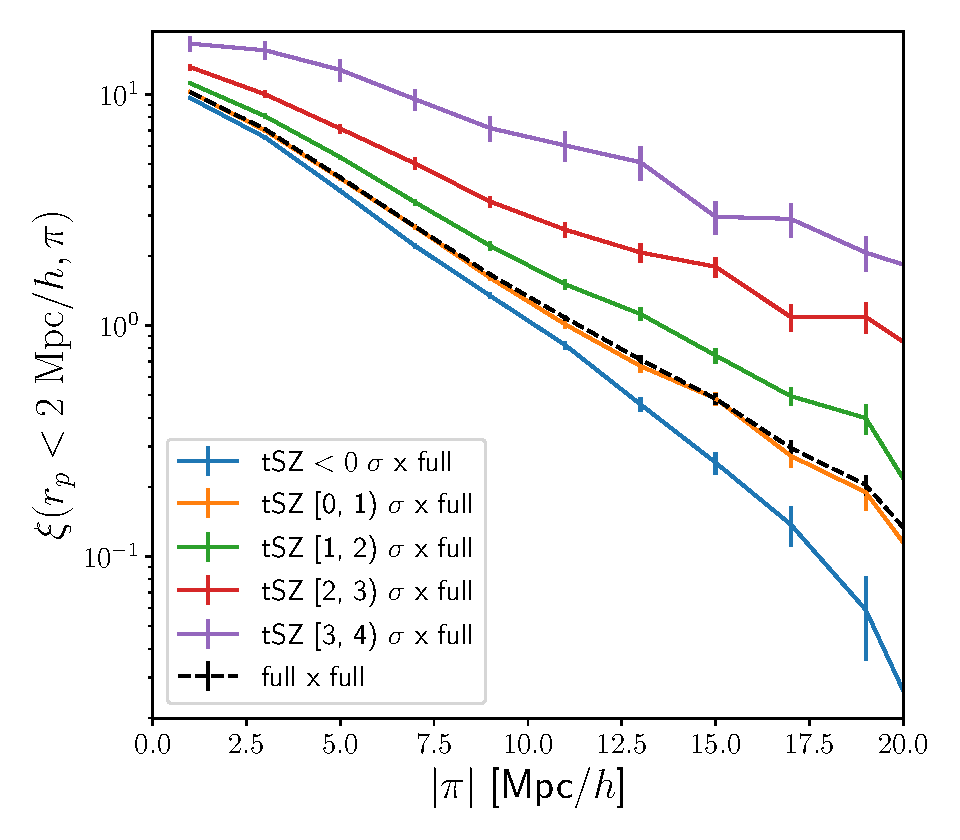
\includegraphics[width=\linewidth]{fig/LRG-z0.4-0.85-SZ-ACTPlanck-filtered2.4-LoS-jack-errorbars.pdf}
    \caption[Small-scale line-of-sight cross-correlation functions of different SNR bins with the full LRG sample]{Small-scale line-of-sight cross-correlation functions of different SNR bins with the full LRG sample.
    There is not only an increase in amplitude, but also a flattening of the slopes of the curves with increasing tSZ SNR, indicating regions with higher tSZ signal have hotter small-scale velocity dispersions.}
    \label{fig:LoS-clustering-SNR-bins}
\end{figure}

To better quantify the slopes, we fit exponentials to the correlation functions:
\begin{equation}
    \xi(\pi) \approx C \exp(-\sqrt{2} \frac{\abs{\pi}}{\sigma_\pi}).
\end{equation}
This is motivated by the exponential fit to the distributions of peculiar radial velocities \citep{Peebles-cosmic-virial-theorem} and a physical Press--Schechter (Gaussian mixture) model \citep{pairwise-peculiar-velocity-distribution-nonlinear}.
$\sigma_\pi$ gives the one-dimensional dispersion (standard deviation).

\begin{figure}[hbtp]
    \centering
    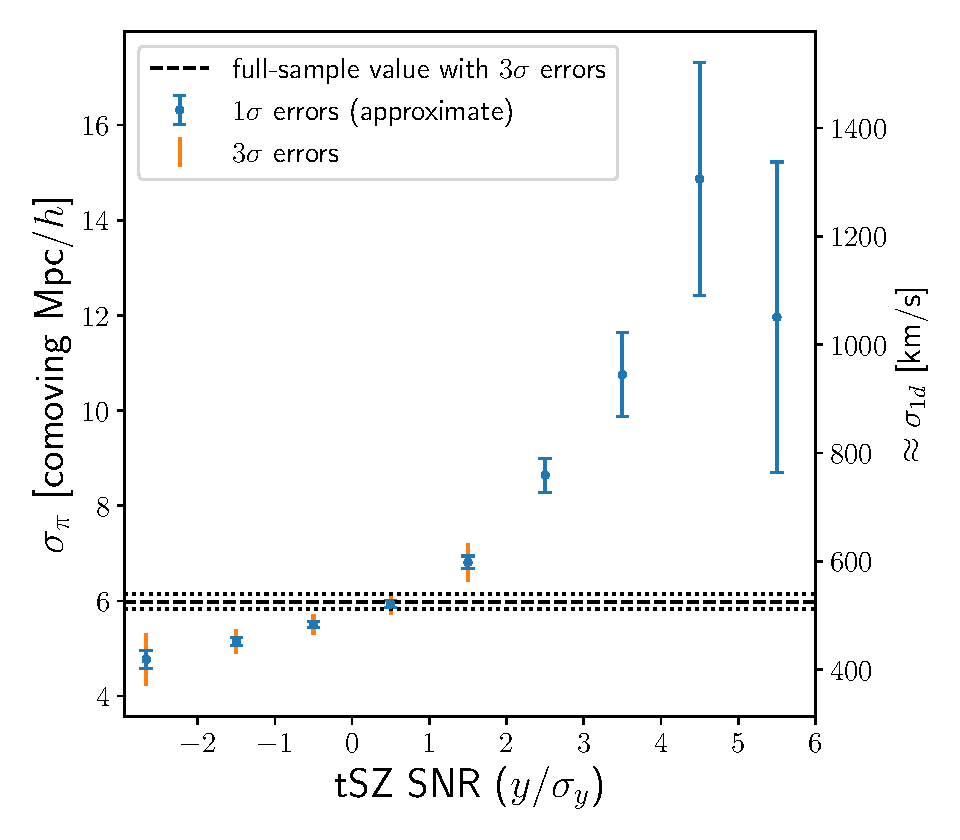
\includegraphics[width=\linewidth]{fig/LRG-z0.4-0.85-SZ-ACTPlanck-filtered2.4-LoS-jack-errorbars-sigmas.pdf}
    \caption[Coordinate and velocity dispersions from small-scale line-of-sight clustering]{One-dimensional comoving coordinate dispersions $\sigma_\pi$ from small-scale line-of-sight clustering.
    Approximate conversion to one-dimensional (line-of-sight) velocity dispersions $\sigma_{1d}$ is provided on the right.
    The dispersion values increase with the signal-to-noise ratio, except the 5 to 6 $\sigma_y$ bin.}
    \label{fig:LoS-sigmas-SNR-bins}
\end{figure}

We plot the fit results for each tSZ SNR bin in \cref{fig:LoS-sigmas-SNR-bins}.
We measure them in comoving line-of-sight separations, but also provide an approximate conversion to line-of-sight peculiar velocities using the average redshift.
The dispersions increase with the tSZ detection level, more significantly for positive values.
The last, 5 to 6 $\sigma_y$ bin, is an exception, although it has a large errorbar.
The 0 to 1 $\sigma_y$ bin is again very close to the average LRG.

Another natural way to summarize \cref{fig:LoS-clustering-SNR-bins} would be by integrating the correlation functions.
This is directly related to the average number of any LRGs in narrow cylinders with axes along the line of sight centered on LRGs belonging in a particular SNR bin.
We provide this summary in \cref{fig:avg-no-close-neighbors-cylinders-SNR-bins}.
The average number of neighbors increases, in accordance with the expectation that LRGs with higher tSZ SNR tend to live in larger clusters.

\begin{figure}[hbtp]
    \centering
    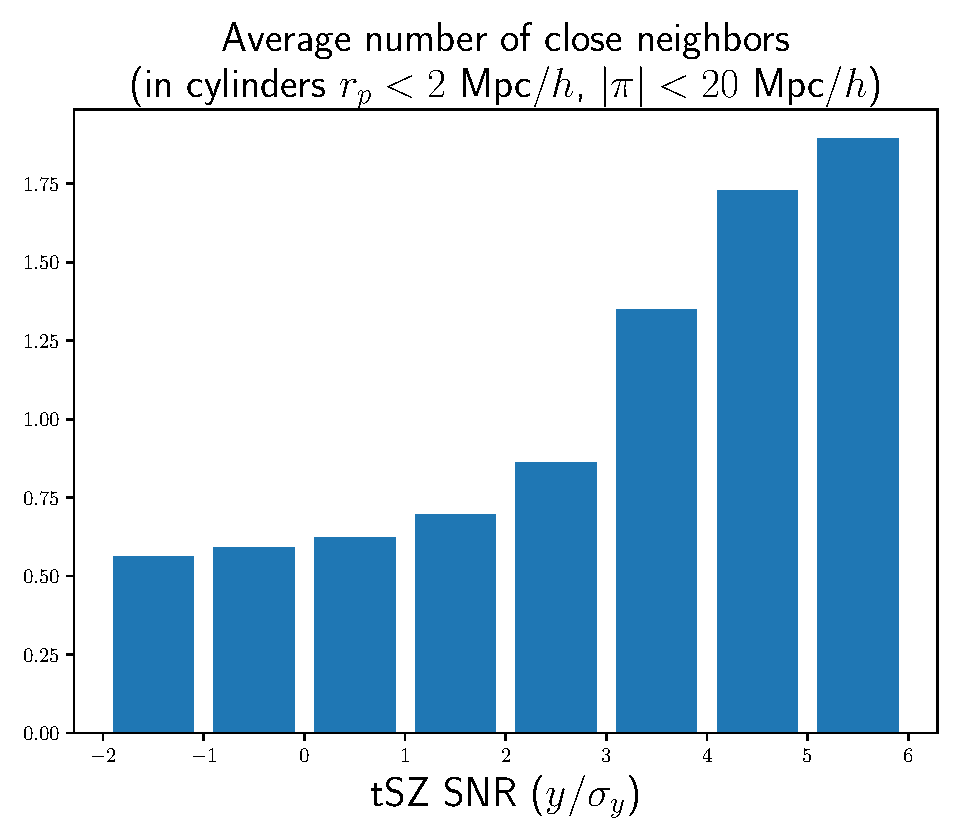
\includegraphics[width=\linewidth]{fig/close_neighbor_counts_cylinders-Y1_rp2_pi20.0-avg-no.pdf}
    \caption[Average number of close neighbors in different tSZ SNR bins]{Average number of close neighbors in different tSZ SNR bins.
    It increases, confirming that stronger tSZ signatures are associated with clusters that have more galaxies.}
    \label{fig:avg-no-close-neighbors-cylinders-SNR-bins}
\end{figure}

We have found even more striking differences in the abundance of galaxies with many neighbors in different SNR bins.
However, it is hard to visualize and interpret more meaningfully.
We provide it in \cref{fig:dist-no-neighbors-cylinders-SNR-bins,sec:close-neighbor-counts-dist} for posterity.

\section{Simulation-based toy model}
\label{sec:DESI-tSZ:mock}

We aim to simulate both galaxy catalogs and $y$ map consistently.
Galaxy catalogs are often made from $N$-body simulations using a halo occupation distribution.
The process has been highly optimized in \abacushod{} \citep{AbacusHOD}.
Therefore we choose to make a Compton parameter map from a halo catalog.

We are aware of the advanced models for SZ-halo connection informed by hydrodynamic simulations or observations \citep[e.g.,][]{simulations-websky,baryon-pasting-algorithm,fast-baryon-painting-Liu}.
However, in this proof-of-concept work, we choose to develop a simpler model that is easier to control.

\subsection{Simple \texorpdfstring{$y$}{y} signal map from an \texorpdfstring{$N$}{N}-body simulation}

The Compton $y$ parameter depends on the electron temperature $T_e(\bm r)$ and number density $n_e(\bm r)$ as functions of spatial position $\bm r$, whereas an $N$-body simulation provides masses and positions of discrete dark matter particles grouped in halos.
Let us recall the theoretical expression for $y$ as the integral along the line of sight \citep{Planck-SZ-map,Sunyaev-Zeldovich-1972}:
\begin{equation} \label{eq:y-parameter}
    y\qty(\bm \theta) = \int_0^{r_{\rm ls}} \frac{k_B T_e\qty(r, \bm \theta)}{m_e c^2} n_e\qty(r, \bm \theta) \sigma_T dr.
\end{equation}
The integral above is taken along the radial coordinate $r$ to the last scattering surface $r_{\rm ls}$, where CMB emerges.
$k_B$ is the Boltzmann's constant, $m_e c^2$ is the electron's rest energy and $\sigma_T$ is the Thomson cross-section.

We estimate electron temperatures $T_e$ using the motions of dark matter particles in halos.
The root-mean-square thermal velocity is analogous to the random velocity dispersion of particles.
The velocity dispersion of dark matter particles belonging to each halo is available in the \abacussummit{} \compaso{} halo catalogs.
The remaining non-trivial step is connecting dark matter to hot gas.
We assume complete ionization, primordial composition\footnote{I.e., mix of hydrogen-1 and helium-4 with the mass fraction of the latter $Y_{\rm He} = 0.2454$ \citep{Planck2018-cosmo}.}, and thermal equilibrium between ions and electrons in the gas.
We find adequate hot gas temperatures\footnote{The 3-dimensional velocity dispersion $\sigma_{3d}\sim 200~{\rm km~s^{-1}}$ yields $T\sim 10^6$~K.} by taking the same kinetic energy of random motions per unit mass as for dark matter particles.

Then, we approximately compute the number of electrons $N_e$ from the dark matter mass.
First, we obtain the baryonic matter mass using the global baryon-to-dark matter ratio given by the cosmic density parameters $\Omega_b/\Omega_{\rm cdm}$.
Second, we estimate the hot gas mass by assuming it constitutes a constant fraction of all baryons $f_{\rm hot}\approx 0.85$.
Finally, we compute the electron number $N_e$ assuming complete ionization of the hot gas and primordial composition as previously.

For simplicity, we use the flat-sky approximation valid for small angular scales.
Accordingly, we switch from $\bm r = \qty(r, \bm \theta)$ decomposition to $\qty(r_\parallel, \bm r_\perp)$:
\begin{equation} \label{eq:y-parameter-flatsky}
    y\qty(\bm r_\perp) \approx \frac{k_B \sigma_T}{m_e c^2} \int_0^{r_{\max}} T_e\qty(r_\parallel, \bm r_\perp) n_e\qty(r_\parallel, \bm r_\perp) dr_\parallel.
\end{equation}

Next, we need to account for particle discreteness.
As the first rough approximation, we take infinitely narrow profiles of $T_e(\bm r) n_e(\bm r)$ for each dark matter particle with the 3-dimensional Dirac delta function $\delta^{(3)}$:
\begin{equation} %\label{} 
    y\qty(\bm r_\perp) \approx \frac{k_B \sigma_T}{m_e c^2} \sum_j \int_0^{r_{\max}} T_{e, j} N_{e, j} \delta^{(3)}\qty(\bm r - \bm r_j) dr_\parallel.
\end{equation}
Here $j$ indexes dark matter particles with positions $\bm r_j$ and the corresponding electron temperature and number estimates.
We can evaluate the integral over $r_\parallel$ by decomposing the delta function in $r_\parallel$ and $r_\perp$\footnote{Namely, $\delta^{(3)}\qty(\bm r - \bm r_j) = \delta^{(1)}\qty(r_\parallel - r_{\parallel, j}) \delta^{(2)}\qty(\bm r_\perp - \bm r_{\perp, j})$. The integral of the former over $dr_\parallel$ gives 1 as long as $r_{\parallel, j}$ is not out of integration bounds.}:
\begin{equation} \label{eq:y-map-discrete-particles} 
    y\qty(\bm r_\perp) \approx \frac{k_B \sigma_T}{m_e c^2} \sum_j T_{e, j} N_{e, j} \delta^{(2)}\qty(\bm r_\perp - \bm r_{\perp, j}).
\end{equation}

In the following step, we need to discretize the $y$ map into pixels.
We can do this by averaging over pixel number $k$ with area $A_k$:
\begin{equation}
    y_k = \frac1{A_k} \int_{A_k} d\bm r_\perp y\qty(\bm r_\perp).
\end{equation}
Substituting \cref{eq:y-map-discrete-particles} into the integral above gives counts of dark matter particles in pixels weighted by their $T_e N_e$ along with constant factors:
\begin{equation}
    y_k = \frac1{A_k} \frac{k_B \sigma_T}{m_e c^2} \sum_{j:\, r_{\perp, j} \in A_k} T_{e, j} N_{e, j}.
\end{equation}

Subsequently, we need to convolve the pixelated map with the point spread function (the CMB instrument beam).
We use fine pixels at this stage.
The common beam for the ACT DR6 + {\it Planck} map has a Gaussian shape with 1.6 arcmin full width at half-maximum \citep{ACT-maps-DR6}.
This translates to $\approx 0.9 \ihMpc$ at $z=0.8$ --- close to the typical halo size.
Thus, the exact width of the electron temperature-density profile is not so important.

Finally, we downsample the map to larger pixels, approximately matching the larger pixel side of 0.5 arcmin in the ACT DR6 + {\it Planck} $y$ map.
Afterwards, we also apply a 2.4 arcmin FWHM Gaussian filter analogously to our data processing.

\subsection{Simple noise model}

First, we have tried to add noise independently for each galaxy.
We have divided the pure $y$ signal produced in the previous section for every galaxy from a galaxy catalog by the $y$ standard deviation.
We take that as the center of the total signal-to-noise ratio distribution.
We assume that the distribution is normal with a standard deviation of 1 (because the value is already normalized by the $y$ standard deviation).
Then, we have computed the contribution of each galaxy to each SNR bin by integrating each Gaussian within bin boundaries (this gives a difference of error functions, which can be evaluated quickly in common libraries).
However, we have found that in this model, the clustering increase with SNR is much stronger than in the data.

Therefore, we implemented realistic spatial correlations in the noise map.
We have done this by generating the noise (normalized by its pixel-wise standard deviations) according to the power spectrum of a noise simulation provided with the ACT DR6 products (accordingly normalized, and filtered\footnote{We applied the filter after normalization by pixel-wise standard deviations (computed previously from 304 realizations of noise simulations). Filtering before normalization corresponds to the data processing more exactly, but it creates small-scale artifacts at the boundaries of regions observed by ACT to different depths.}).
We also produce a periodic square $y$ standard deviation map, in which the same values occupy the same fractions of the area as for ACT DR6 + {\it Planck}.
To obtain the total signal-to-noise ratio, we add the normalized noise to the ratio of the pure signal to the standard deviation, all taken from the pixel to which a mock galaxy falls.

By construction, our final mock noise map is independent of the mock signal.
This might not be true in actual data processing (deprojection of different foregrounds) and may account for some of the differences we notice later.

\subsection{Calibration}

To refine our arbitrary coefficients in the $y$ signal making described above, we rescale the signal to match the 3-dimensional density of $>4\sigma$ detections (cluster candidates) in the data ($0.4<z<0.85$).
This should be good as long as there is rarely more than one significant SZ cluster per pixel.
Otherwise, we would need to match depth with the real Universe, which would be challenging with cut-sky mocks as well, because it would require bigger simulation boxes.

We match the 5711 peaks ($>4\sigma$) detected in the ACT DR6 + {\it Planck} tSZ $y$ map after our fiducial filtering to the ACT DR5 SZ cluster catalog \citep{ACT-SZ-clusters-DR5} containing 4195 confirmed objects.
Because of the differences in data and cluster candidate detection methods, the matching is not 1-to-1.
We restrict good matches to 2285 unique clusters within 2.4 arcmin of our peaks, among which 1179 belong to our redshift range ($0.4<z<0.85$).
Given the sky area of the ACT DR5 cluster search mask, their average density is $\approx 40 \qty(\ihGpc)^{-3}$.
From this, we extrapolate the density of our $>4\sigma$ peaks as $\approx 100 \qty(\ihGpc)^{-3}$.
We rescale the mock $y$ signal to match this density of $>4\sigma$ peaks in our first map (given that our simulation box is $\qty(2\ihGpc)^3$).
The resulting signal rescaling factor is $\approx 1.14$, which suggests that our rough assumptions were not far off.

It is important to take noise into account in this calibration: without noise, we find the rescaling factor $\approx 1.59$.
We do not assume that the noise distribution is asymmetric, but higher signals are rarer\footnote{That said, true negative signals are not possible in our simplistic model, and are probably hard to achieve in reality.}.
Therefore, at a given final signal-to-noise\footnote{At least a positive value.}, more objects were shifted ``up'' by noise (have a smaller true signal) than ``down'' (from a larger true signal).

\subsection{Mock clustering}

\begin{figure}[htbp]
    \centering
    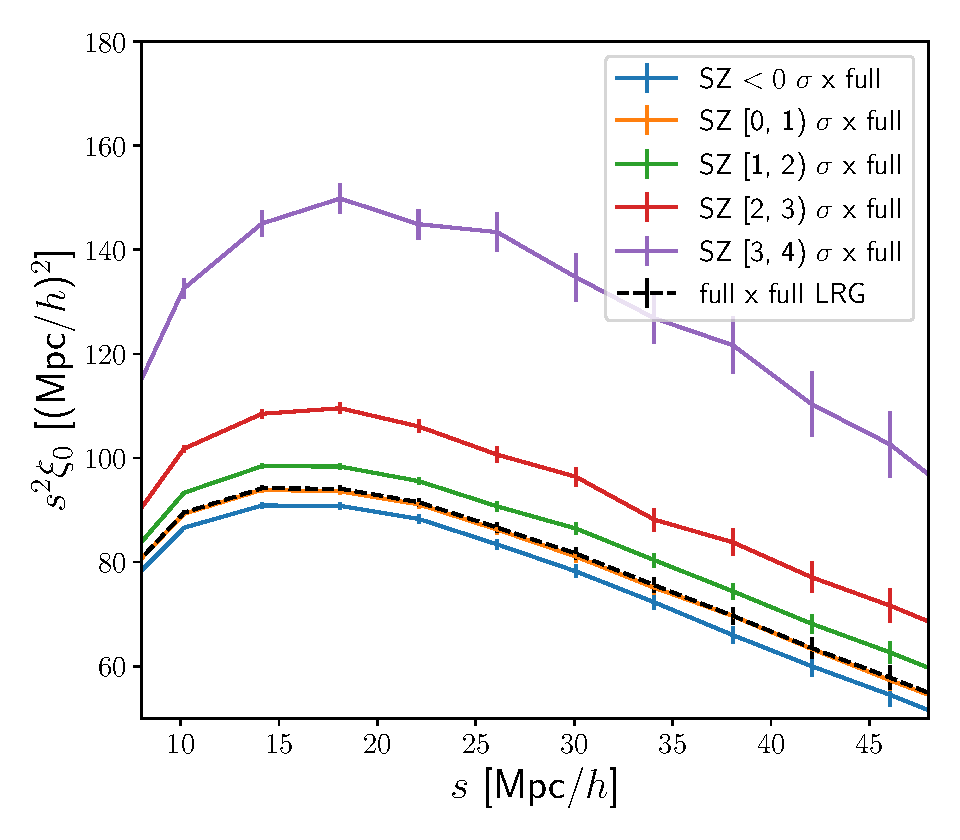
\includegraphics[width=\linewidth]{fig/LRG-cubic-SZ-ACTPlanck-filtered2.4-monopole-jack-errorbars.pdf}
    \caption[Mock large-scale cross-correlation function of different SNR bins with the full LRG sample]{Mock large-scale cross-correlation function of different SNR bins with the full LRG sample.
    Similarly to the data (\cref{fig:clustering-SNR-bins}), the clustering is enhanced at higher SNR, but more slowly.
    Also note that the $[0, 1)$ $\sigma$ bin remains very similar to the full sample.}
    \label{fig:mock-clustering-SNR-bins}
\end{figure}

Bringing together all the ingredients, we can finally compare the clustering of SNR bins in mocks to data.
We focus on the larger scales, showing full cross-correlation functions in \cref{fig:mock-clustering-SNR-bins} and relative galaxy bias in \cref{fig:mock-relbias-SNR-bins}.
We see a clustering/bias enhancement trend generally similar to the data, although the increase appears to be slower near zero signal and faster at high signal.
As we mentioned before, one of the reasons for the difference may be the independence of noise and signal in our mocks.

\begin{figure}[htbp]
    \centering
    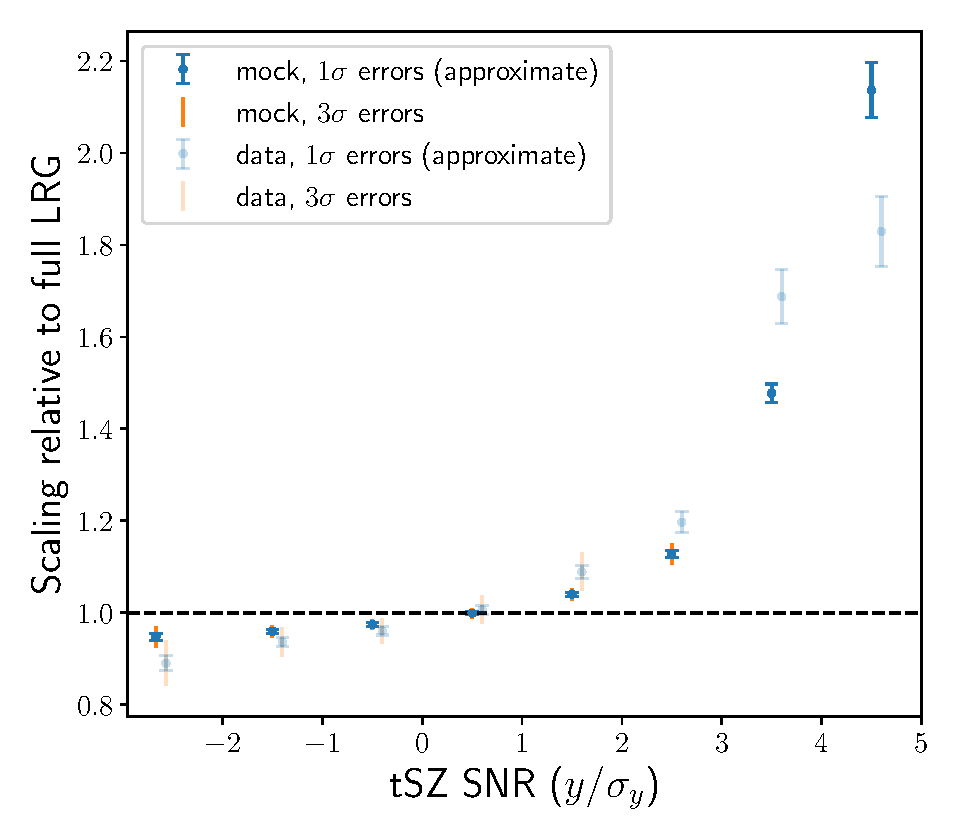
\includegraphics[width=\textwidth]{fig/LRG-cubic-SZ-ACTPlanck-filtered2.4-monopole-jack-errorbars-relbias-with-data.pdf}
    \caption[Mock galaxy bias of different SNR bins relative to the full LRG sample]{Mock galaxy bias of different SNR bins relative to the full LRG sample.
    Similarly to data (shaded and shifted slightly to the right for clarity), the relative bias increases with the SNR, but less rapidly near 0 and then more steeply at higher values.}
    \label{fig:mock-relbias-SNR-bins}
\end{figure}

Our next step will be to investigate how the differences in the clustering of SNR bins react to changes in halo occupation distribution parameters.
Doing this with all cross-correlation functions (\cref{fig:mock-clustering-SNR-bins}) is hardly viable, because it would add even more lines to the plot, making it hard to interpret.
The relative bias plot (\cref{fig:mock-relbias-SNR-bins}) provides a cleaner way forward.

Currently, we do not focus on the small-scale line-of-sight clustering (analogs of \cref{fig:LoS-clustering-SNR-bins,fig:LoS-sigmas-SNR-bins}).
One of the reasons is that we do not model fiber assignment in our cubic mocks for simplicity.
On large scales, the fiber assignment incompleteness effects can be mitigated quite well with weights \citep{KP3s6-Bianchi,DESI2024.II.KP3}, but on small scales it is a much more difficult problem.

\subsection{Relating halo mass to thermal Sunyaev-Zeldovich signatures}

Simulations also allow us to access the true halo properties, unlike the data.
With this, we can explore connections with SZ properties (bearing in mind they are produced approximately).

We present mock correlations between halo mass and the noiseless tSZ $y$ signal (left) or the final tSZ signal-to-noise ratio (right; both in their central pixels) in \cref{fig:Mhalo-tSZ-relations-mocks}.
We count halo contributions by their mass\footnote{In numbers, small halos strongly dominate, making such plots less informative in our opinion.} to minimize assumptions about the galaxy-halo connection.
When we have better constraints on the halo occupation distribution, we can count the number of galaxies, which is non-linear in halo mass.
We see a wide range of tSZ observables for smaller halo masses, but the most massive halos can be identified with the highest signal or signal-to-noise.
Furthermore, the noiseless signal might have a power-law relation with halo mass, whereas the smearing towards smaller halo masses might be caused by such halos appearing in the same lines of sight as larger halos (within the point spread function).

\begin{figure}[htbp]
    \centering
    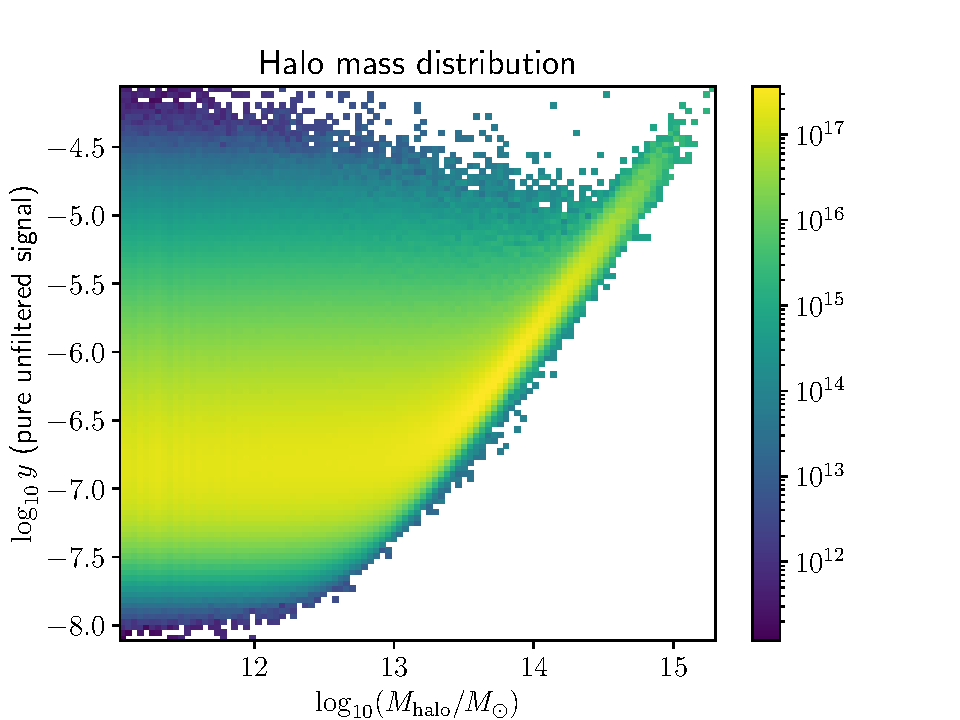
\includegraphics[width=0.495\linewidth]{fig/Mhalo-y-unfiltered-unscaled.pdf}
    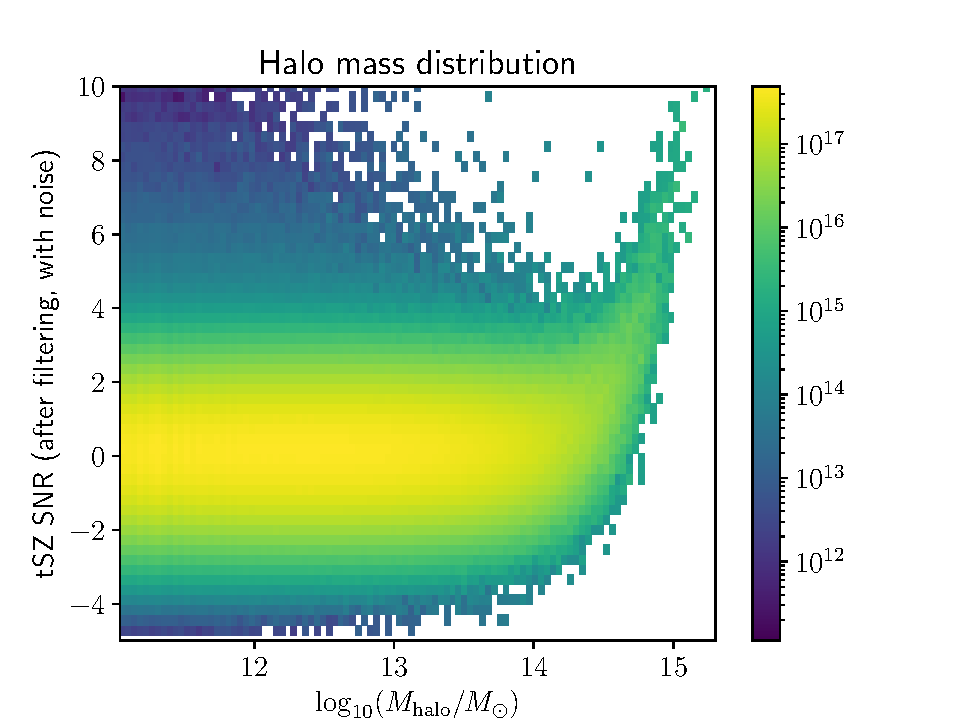
\includegraphics[width=0.495\linewidth]{fig/Mhalo-SNR-filtered.pdf}
    \caption[Correlations between halo mass and tSZ observables in our simulation-based model]{Histograms displaying correlations between halo mass and tSZ quantities in the corresponding pixels in our mock map.
    Left: noiseless $y$ parameter.
    Right: SNR including our simplistic noise.
    Histograms are weighted by halo mass to minimize dependence on galaxy-halo connection assumptions.}
    \label{fig:Mhalo-tSZ-relations-mocks}
\end{figure}

A well-known or calibrated halo mass to tSZ observables relation can be used to make theoretical predictions about clustering, particularly on larger scales.
Furthermore, if this relation is less dependent on cosmology than halo mass-density relations, it would enable more robust cosmological inference beyond the 2-point function.

Alternatively, it is possible to build a simulation-based model after investing in a large number of high-quality mocks \citep[like for density-split clustering in][]{density-split-clustering-sim-based-model}.
This is a long way from our toy model.
More generally, we are concerned about robustness, whether one can simulate SZ from first principles well enough.

\section{Conclusions}
\label{sec:DESI-tSZ:conclusions}

We demonstrate that there is valuable cosmological information in the thermal Sunyaev-Zeldovich (tSZ) map in the ``noise'' beyond the individual cluster candidates.
Soon, we aim to quantify the sensitivity of our effects to the galaxy-halo connection using the halo simulations.
In further work, we are going to investigate constraining the growth of structure.

From large-scale clustering, we find that a higher tSZ signal-to-noise ratio corresponds to galaxies with a higher bias (\cref{fig:relbias-SNR-bins}).
This can allow us to select luminous red galaxy sub-samples and test their structural consistency \citep[e.g., following][]{LSS-color-dependent-stochasticity},
or better understand their biases to better constrain primordial non-Gaussianity \citep[in the spirit of][]{multi-tracer-PNG-forecasts}.

From small-scale line-of-sight clustering, we find that the velocity dispersion increases considerably with tSZ SNR (\cref{fig:LoS-sigmas-SNR-bins}).
This is likely a clean indication of strong non-perturbative non-linearities (Fingers of God) which can be removed to improve the theoretical modeling \citep{removing-FoG}.

We also see that galaxies with higher SNR bins have higher numbers of close neighbors (\cref{fig:avg-no-close-neighbors-cylinders-SNR-bins}).
This could help inform the galaxy multiplet studies \citep[e.g.][]{DESI-galaxy-multiplets-tidal-field}.

We have built a simple mock tSZ map that allowed us to reproduce general trends from the data (\cref{fig:mock-clustering-SNR-bins,fig:mock-relbias-SNR-bins}).
However, we note differences, and investigating their causes will be our next priority.

Eventually, we hope to use a relatively small number of simulations to calibrate the relation between the halo mass and the Sunyaev-Zeldovich observables and build a semi-analytical model of galaxy subsample clustering.
Alternatively, one can invest in a large number of accurate simulations with different cosmological and galaxy-halo connection parameters to build a simulation-based model or inference pipeline like for density-split \citep{density-split-clustering-sim-based-model} or density-marked clustering \citep{density-marked-PS-SBI}.

Combining 3D galaxy surveys and Sunyaev-Zeldovich data is very promising.
As well as the number of spectra with DESI, the SZ measurements are improving rapidly with the current and next CMB experiments like Simons Observatory \citep{SO} and CMB-S4 \citep{CMBS4,CMBS4white}.
Joint analysis of different measurements has high potential to improve our measurements and uncover new tensions.

\section*{Acknowledgments}

MR and DJE are supported by U.S. Department of Energy grant DE-SC0013718 and as a Simons Foundation Investigator.

This material is based upon work supported by the U.S. Department of Energy (DOE), Office of Science, Office of High-Energy Physics, under Contract No. DE–AC02–05CH11231, and by the National Energy Research Scientific Computing Center, a DOE Office of Science User Facility under the same contract. Additional support for DESI was provided by the U.S. National Science Foundation (NSF), Division of Astronomical Sciences under Contract No. AST-0950945 to the NSF National Optical-Infrared Astronomy Research Laboratory; the Science and Technology Facilities Council of the United Kingdom; the Gordon and Betty Moore Foundation; the Heising-Simons Foundation; the French Alternative Energies and Atomic Energy Commission (CEA); the National Council of Humanities, Science and Technology of Mexico (CONAHCYT); the Ministry of Science and Innovation of Spain (MICINN), and by the DESI Member Institutions: \url{https://www.desi.lbl.gov/collaborating-institutions}. Any opinions, findings, and conclusions or recommendations expressed in this material are those of the author(s) and do not necessarily reflect the views of the U. S. National Science Foundation, the U. S. Department of Energy, or any of the listed funding agencies.

The authors are honored to be permitted to conduct scientific research on Iolkam Du’ag (Kitt Peak), a mountain with particular significance to the Tohono O’odham Nation.

This work has used the following software packages: \textsc{astropy} \citep{astropy:2013, astropy:2018, astropy:2022}, \textsc{Jupyter} \citep{2007CSE.....9c..21P, kluyver2016jupyter}, \textsc{matplotlib} \citep{Hunter:2007}, \textsc{numpy} \citep{numpy}, \pycorr{} \citep{pycorr,corrfunc-1,corrfunc-2}, \textsc{python} \citep{python}, \textsc{scipy} \citep{2020SciPy-NMeth, scipy_8092679}, and \textsc{scikit-learn} \citep{scikit-learn, sklearn_api, scikit-learn_10034229}.

This research has made use of NASA's Astrophysics Data System.
Software citation information has been aggregated using \texttt{\href{https://www.tomwagg.com/software-citation-station/}{The Software Citation Station}} \citep{software-citation-station-paper, software-citation-station-zenodo}.